\chapter[Annealing and adiabatic computation]{Optimization, annealing and adiabatic quantum computation}\label{ch:annealing}

Many practical problems can be formulated as the minimization of a cost function: fitting a model to data, scheduling, routing, or finding the ground state of a physical system. When the variables are discrete,
the number of possible configurations grows exponentially with the number of variables, and many such problems are NP-hard. In this chapter we show how an optimization problem can be cast in a form suitable for
a special kind of quantum computer, the \emph{quantum annealer}, how quantum annealing compares with its classical counterpart, simulated annealing, and how both relate to \emph{adiabatic quantum computation}.

\section{Linear regression as a binary optimization problem}
\subsection{Classical linear regression}
Consider a dataset of $N$ entries, each described by $d$ features $x_1,\dots,x_d$, together with $N$ labels $y$. Linear regression looks for the weights $w_0,\dots,w_d$ of the linear model
\begin{equation}
  y=w_0+w_1x_1+w_2x_2+\dots+w_dx_d .
\end{equation}
Adding a constant feature $x_0=1$ for the bias $w_0$, the dataset becomes an $N\times D$ matrix $X$ with $D=d+1$ columns, and the model reads $y=Xw$. The standard classical method, \emph{ordinary least squares},
minimizes the squared error
\begin{equation}
  E(w)=\norm{Xw-y}^2=w^TX^TXw-2w^TX^Ty+y^Ty.
\end{equation}
The minimum satisfies $\nabla E=2X^T(Xw-y)=0$ (the \emph{normal equations}), which gives the closed-form solution
\begin{equation}
  w=(X^TX)^{-1}X^Ty.
\end{equation}
The bottleneck is the inversion of the $D\times D$ matrix $X^TX$, which costs $\order(D^3)$ operations (forming $X^TX$ itself costs $\order(ND^2)$). For large problems, approximate iterative methods are used instead,
such as gradient descent, $w\to w-\alpha\nabla E(w)$, where $\alpha$ is the learning rate. Since $E$ is a convex quadratic function, gradient descent converges to the global minimum for small enough $\alpha$.

\subsection{The QUBO formulation}
Quantum annealers solve a specific class of problems, \emph{quadratic unconstrained binary optimization} (QUBO):
\begin{equation}\label{eq:qubo}
  \min_{z\in\{0,1\}^M}z^TAz+z^Tb,
\end{equation}
where $z$ is a vector of $M$ binary variables, $A\in\R^{M\times M}$ is the QUBO matrix and $b\in\R^M$ the QUBO vector. (Since $z_i^2=z_i$, the linear term can be absorbed in the diagonal of $A$.)
To bring linear regression into this form \cite{DatePotok2021}, note that $E(w)$ is already quadratic, but the weights are real numbers, not binary variables. We therefore \emph{binarize} them: each weight is
approximated by a combination of $K$ binary variables $\hat w_{ik}\in\{0,1\}$,
\begin{equation}
  w_i=\sum_{k=1}^Kp_k\hat w_{ik},
\end{equation}
where the precision vector $p=(p_1,\dots,p_K)^T$ fixes the values that can be represented. For example, $p=(0.25,0.5)^T$ allows $w_i\in\{0,0.25,0.5,0.75\}$; negative values are obtained with negative entries of $p$
(e.g.\ $p=(-1,0.5,0.25)$). Collecting all binary variables into a single vector of length $DK$, $\hat w=(\hat w_{11},\dots,\hat w_{1K},\dots,\hat w_{D1},\dots,\hat w_{DK})^T$, and defining the $D\times DK$ precision
matrix $P=I_D\otimes p^T$, we have $w=P\hat w$. Substituting and discarding the constant $y^Ty$,
\begin{equation}
  \min_{\hat w\in\{0,1\}^{DK}}E(\hat w)=\hat w^TP^TX^TXP\hat w-2\hat w^TP^TX^Ty.
\end{equation}
This is exactly the QUBO problem \cref{eq:qubo} with $z=\hat w$, $A=P^TX^TXP$, $b=-2P^TX^Ty$. The number of binary variables, $DK$, does not depend on the number of data points $N$: the dataset enters only through
$X^TX$ and $X^Ty$.

\paragraph{Performance.} Date and Potok \cite{DatePotok2021} implemented this approach on a D-Wave 2000Q quantum annealer and compared it with the Scikit-learn library on an 8-core Intel i9 workstation. They obtained a
speed-up of up to 2.8 for the largest dataset, with about $16.8\times10^6$ data points, and comparable regression errors. The size of the problem was limited by the hardware: the D-Wave 2000Q can handle at most 64
binary variables with all-to-all connectivity, so with $K=2$ bits per weight the number of features was limited to $D\le32$. Such results depend strongly on the specific hardware and software used, and should not be
read as a general quantum advantage: the regression problem is convex and is solved exactly in polynomial time classically.

\section{Simulated annealing}
QUBO problems are hard in general, and heuristic methods are widely used. One of the most successful is \emph{simulated annealing} (SA) \cite{Kirkpatrick1983}, based on the Metropolis algorithm of statistical physics.
It mimics the slow cooling (annealing) of a material, which allows the atoms to settle into a low-energy crystal instead of a disordered glass.

To minimize a function $f$ of $n$ variables, SA performs a random walk in configuration space, $x_{\rm init}\to x_1\to x_2\to\cdots$. At each step a random change of the configuration is proposed (e.g.\ flipping one bit).
Let $\Delta=f(x_{i+1})-f(x_i)$ be the resulting change of the cost function. The move is accepted with the \emph{Metropolis probability}
\begin{equation}\label{eq:metropolis}
  \mathrm{Prob(accept)}=\min\left(1,\e^{-\Delta/T}\right).
\end{equation}
A move that lowers the cost ($\Delta<0$) is always accepted. A move that raises it is accepted with probability $\e^{-\Delta/T}<1$, which allows the walker to climb out of local minima (\cref{fig:annealing}).

\begin{origin}[: why the Metropolis rule?]
The rule is designed so that the random walk samples the Boltzmann distribution $\pi(x)\propto\e^{-f(x)/T}$ of a physical system with energy $f$ at temperature $T$. A Markov chain with transition probabilities $W(x\to y)$
has $\pi$ as stationary distribution if it satisfies \emph{detailed balance}, $\pi(x)W(x\to y)=\pi(y)W(y\to x)$. With symmetric proposals, \cref{eq:metropolis} gives
$W(x\to y)/W(y\to x)=\e^{-(f(y)-f(x))/T}=\pi(y)/\pi(x)$. As $T\to0$, $\pi$ concentrates on the global minima. The difficulty is that at low $T$ the walk becomes trapped behind barriers, for a time
$\sim\e^{\Delta_{\rm barrier}/T}$ (Arrhenius law).
\end{origin}
The parameter $T$ plays the role of a temperature. It is slowly decreased during the search, so that the walker first explores the landscape broadly and then settles into a deep minimum. If the temperature is lowered slowly
enough, for instance as $T(i)=a/\ln i$ with a sufficiently large constant $a$ (of the order of the largest barrier), the algorithm is guaranteed to find the global minimum with probability approaching one \cite{Geman1984}.
Such a slow schedule is impractical, however, and faster schedules are used in practice, without guarantee.

\begin{figure}[h]\centering
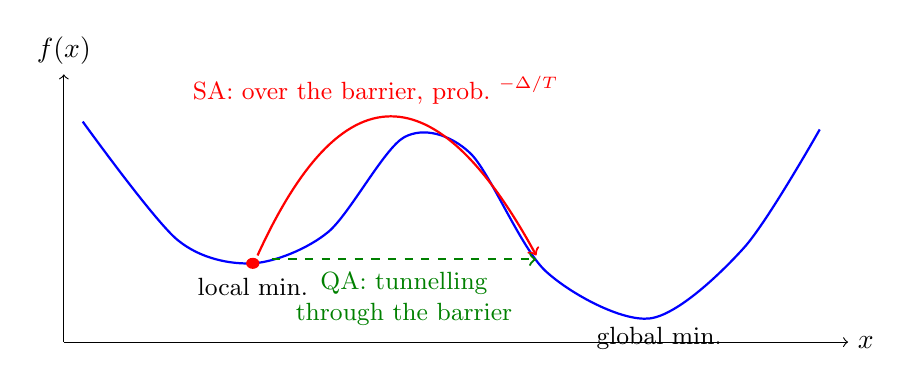
\begin{tikzpicture}[xscale=1.2]
  \draw[->] (0,0)--(8.3,0) node[right]{$x$};
  \draw[->] (0,0)--(0,3.4) node[above]{$f(x)$};
  \draw[thick,blue] plot[smooth] coordinates {(0.2,2.8) (1.2,1.3) (2.0,1.0) (2.8,1.4) (3.6,2.6) (4.3,2.4) (5.1,0.9) (6.2,0.3) (7.2,1.2) (8,2.7)};
  \fill[red] (2.0,1.0) circle (2pt);
  \draw[->,red,thick] (2.05,1.1) .. controls (3,3.6) and (4,3.3) .. (5.0,1.1);
  \node[red,align=center,font=\small] at (3.3,3.2) {SA: over the barrier, prob.\ $\e^{-\Delta/T}$};
  \draw[->,green!50!black,thick,dashed] (2.2,1.05)--(5.0,1.05);
  \node[green!50!black,font=\small,align=center] at (3.6,0.55) {QA: tunnelling\\through the barrier};
  \node[font=\small] at (2.0,0.7) {local min.};
  \node[font=\small] at (6.3,0.05) {global min.};
\end{tikzpicture}
\caption{Escaping from a local minimum. In simulated annealing the walker must climb over the barrier by thermal activation. In quantum annealing it can also tunnel through it.}\label{fig:annealing}
\end{figure}

\section{Quantum annealing}
In quantum annealing (QA) \cite{Kadowaki1998}, the thermal fluctuations of simulated annealing are replaced by \emph{quantum fluctuations}. The cost function is encoded in a Hamiltonian $H_F$, the final Hamiltonian, whose
ground state is the solution. A second, ``disordering'' Hamiltonian $H_D$ is added, with a time-dependent strength $\Gamma(t)$:
\begin{equation}
  H(t)=H_F+\Gamma(t)H_D .
\end{equation}
The role of the temperature $T$ is now played by $\Gamma$, which is slowly decreased to zero. The essential requirement is that the two Hamiltonians do not commute, $[H_D,H_F]\neq0$, just as the position $x$ and momentum $p$
of a particle do not commute. The disordering term plays the role of a kinetic energy. It makes the system move in configuration space, and allows it to tunnel through energy barriers instead of climbing over them.
In practice $H_D$ is usually a transverse field, $H_D=-\sum_i\sigma^x_i$, which does not commute with the $\sigma^z$ operators of the cost Hamiltonian. Its ground state, the equal superposition of all configurations, is
the starting point of the evolution.

\paragraph{Tunnelling vs thermal activation.} For a barrier of height $\Delta$ and width $w$, thermal activation has a rate $\propto\e^{-\Delta/T}$, independent of $w$. Quantum tunnelling of a particle of mass $m$ has the
WKB rate $\propto\exp(-\frac{2}{\hbar}\int\sqrt{2m(V-E)}\dd x)\sim\exp(-w\sqrt{2m\Delta}/\hbar)$, which depends on $\sqrt\Delta$ and on $w$. Tunnelling therefore wins for \emph{tall but narrow} barriers, and loses
for wide ones. In a spin system, the ``width'' is the number of spins that must flip together (Hamming distance), and the transverse field must couple configurations through many orders of perturbation theory.

Convergence can also be guaranteed for quantum annealing. If the transverse field decreases as $\Gamma(i)\ge b/(i+1)^{c/n}$, where $b$ and $c$ are constants and $n$ is the number of variables, the system reaches the ground
state with probability approaching one \cite{MoritaNishimori2008}. This power-law schedule is much faster than the logarithmic schedule required by simulated annealing. In practice, however, little is known about the best
choice of $H_D$ or of the schedule $\Gamma(t)$, and whether quantum annealing offers a general speed-up over the best classical methods remains an open question.

\section{The Ising model}
\begin{origin}[: the Ising model]
The Ising model was proposed by W.~Lenz (1920) and solved in one dimension by his student E.~Ising (1925) as a model of ferromagnetism. Each site carries a magnetic moment that can point up or down, $s_i=\pm1$.
Neighbouring moments interact through the exchange interaction, a consequence of the Pauli principle and the Coulomb repulsion between electrons (\cref{sec:spinqubits}), which favours parallel ($J<0$ in the convention below) or
antiparallel ($J>0$) alignment; a magnetic field acts on each moment. In a strongly anisotropic magnet only the $z$ components matter, and the Heisenberg interaction $J\vec S_i\cdot\vec S_j$ reduces to $JS_i^zS_j^z$.
With random couplings of both signs, the model describes \emph{spin glasses}, whose rugged energy landscape, with exponentially many local minima, is the archetype of hard optimization problems.
\end{origin}
The cost Hamiltonian of a quantum annealer is that of an Ising model, a set of spins $s_i=\pm1$ with energy
\begin{equation}
  H=\sum_ih_is_i+\sum_{i<j}J_{ij}s_is_j,
\end{equation}
where $h_i$ are local fields and $J_{ij}$ are couplings ($J_{ij}<0$ favours parallel spins, i.e.\ ferromagnetic order). The task is to find the ground state, the spin configuration of lowest energy. For spins on a
$d$-dimensional grid this is easy in special cases (e.g.\ planar graphs without fields can be solved in polynomial time) but NP-hard in general, already for a two-dimensional grid with non-zero fields $h_i$ \cite{Barahona1982}.
On a quantum annealer, the spins are qubits and the Hamiltonian is
\begin{equation}
  H_{\rm Ising}=\sum_ih_i\sigma_i^z+\sum_{i<j}J_{ij}\sigma_i^z\sigma_j^z .
\end{equation}
It is diagonal in the computational basis: each basis state $\ket{s_1\dots s_n}$ is an eigenstate with eigenvalue $H(s)$.

\section{From optimization problems to the Ising model}
Many optimization problems can be mapped onto the Ising model \cite{Lucas2014}. The most direct is QUBO: given weights $Q_{ij}$, assign binary values $x_i\in\{0,1\}$ to minimize
\begin{equation}
  f_{\rm QUBO}(x)=\sum_{i\le j}Q_{ij}x_ix_j .
\end{equation}
The change of variables $s_i=1-2x_i$, i.e.\ $x_i=(1-s_i)/2$, transforms this into an Ising energy. For the diagonal terms, $x_i^2=x_i$ and $Q_{ii}x_i=\frac{Q_{ii}}2-\frac{Q_{ii}}2s_i$. For $i<j$,
\begin{equation}
  Q_{ij}x_ix_j=\frac{Q_{ij}}4\left(1-s_i-s_j+s_is_j\right).
\end{equation}
Collecting the terms,
\begin{equation}
  J_{ij}=\frac{Q_{ij}}4,\qquad h_i=-\frac{Q_{ii}}2-\frac14\sum_{j\neq i}Q_{ij},
\end{equation}
up to an irrelevant constant, where $Q_{ij}$ with $j<i$ stands for $Q_{ji}$. The linear regression problem of the previous section can thus be solved on a quantum annealer.

\paragraph{MAX-2-SAT.} Another example is weighted MAX-2-SAT, a satisfiability problem. We are given $m$ clauses, each containing two Boolean variables or their negations, for example $C_i=(l_{i1}\vee l_{i2})$, and each with a
weight $w_i$. The goal is to find the assignment that maximizes the total weight of the satisfied clauses. A clause is violated only if both of its literals are false. Writing the literals as binary variables (a negated variable
$\bar x$ is $1-x$), its penalty $w_i(1-l_{i1})(1-l_{i2})$ is quadratic, so the problem is again a QUBO, and with $s_i=1-2x_i$ an Ising problem.

\paragraph{Constraints.} Constraints are added as quadratic penalties. For example, ``exactly one of $x_1,\dots,x_k$ is 1'' becomes the penalty $\lambda(1-\sum_ix_i)^2$, with $\lambda$ larger than the scale of the cost function
(this is how the travelling salesman problem is mapped onto QUBO, with $n^2$ variables $x_{c,t}$ = ``city $c$ visited at time $t$'').

\section{Quantum annealers in practice}
The best-known quantum annealers are built by D-Wave with superconducting flux qubits (\cref{sec:transmon}), in which the two directions of a persistent current play the role of $s=\pm1$, and the transverse field is a tunnelling
between them. The D-Wave Advantage system has more than 5000 qubits, each coupled to up to 15 others, with more than 35\,000 couplers in total. Since the hardware graph is not fully connected, a general problem must first be
\emph{embedded}: a logical variable that interacts with many others is represented by a chain of physical qubits, strongly coupled ferromagnetically so that they behave as one. A fully connected problem of $n$ variables needs
$\order(n^2)$ physical qubits. This limits the size of problems with dense interactions, as in the linear regression example above. The annealer operates at about $15$\,mK, but the annealing time ($\mu$s) is long compared with
$T_2$ (ns), so it is an open quantum system at finite temperature, not a coherent adiabatic computer.

As an example of a realistic application, quantum annealing has been applied to optimization problems for constellations of low-Earth-orbit satellites. The problem is written as a QUBO, converted into an Ising model and solved
on the D-Wave Advantage, and the results are compared with simulated annealing on a classical laptop processor. A notable observation in comparisons of this kind is that quantum annealing finds many local valleys of the cost
function that are missed by simulated annealing \cite{Koshka2019}. These are not the global optimum, but they can be useful near-optimal solutions, or useful samples for applications such as machine learning.

\section{Adiabatic quantum computation}
\subsection{Optimization problems}
Adiabatic quantum computation (AQC) \cite{Farhi2001} is designed to solve optimization problems of the type introduced above. We are given an objective function $f:D^n\to\R$ of $n$ variables taking values in a discrete domain $D$,
and we must find the configuration $\vec x$ that minimizes $f(\vec x)$. We consider only unconstrained problems. Two examples illustrate how general this formulation is.

\paragraph{Boolean satisfiability (SAT).} SAT was the first problem proven to be NP-complete \cite{Cook1971}. A Boolean formula of $n$ variables is given as a conjunction of $m$ clauses, $B(x)=\bigwedge_{c=1}^mC_c$, and we look for
an assignment $x$ for which $B(x)$ is true. To turn this into an optimization problem, we associate with each clause a function $f_c(x)$ with $f_c(x)=0$ if $C_c$ is satisfied by $x$, and $f_c(x)\ge1$ otherwise, and minimize
\begin{equation}
  f_{\rm CNF}(x)=\sum_{c=1}^mf_c(x).
\end{equation}
The logical product $\wedge$ has become a sum because each $f_c$ measures the violation of its clause. The formula is satisfiable if and only if the minimum of $f_{\rm CNF}$ is zero.

\paragraph{Factoring.} Given an integer $N$, find integers $x,y>1$ that minimize $f_N(x,y)=(N-xy)^2$. The minimum is zero iff $N=xy$. (Writing $x,y$ in binary gives a polynomial of degree 4 in the bits, which can be reduced to
a quadratic one with auxiliary variables. This approach has no known speed-up, unlike Shor's algorithm.)

\subsection{The adiabatic algorithm}
An AQC algorithm uses a register of $n$ qubits in a state $\ket{\phi_t}$ that evolves under a time-dependent Hamiltonian $H(t)$ with the following properties.
\begin{enumerate}
  \item The initial Hamiltonian $H_I$ has a ground state that is easy to find and to prepare.
  \item The final, or problem, Hamiltonian $H_F$ is such that its ground state, $H_F\ket{S_{\rm ground}}=E_F\ket{S_{\rm ground}}$ with the minimal eigenvalue, is the basis state $\ket x$ that minimizes $f$.
  \item An evolution path $s(t)$ goes from 1 to 0 as $t$ goes from 0 to the final time $t_f$, for example linearly, $s(t)=1-t/t_f$, with
  \begin{equation}
    H(t)=s(t)H_I+\left(1-s(t)\right)H_F .
  \end{equation}
\end{enumerate}
The system is prepared in the ground state of $H_I$, and the Hamiltonian is slowly changed into $H_F$. If the change is slow enough, the system remains in the instantaneous ground state, and at $t=t_f$ it is in the ground state of $H_F$.
A measurement in the computational basis then gives the solution.

The linear interpolation is not necessarily the best choice. A curved path in the space of Hamiltonians, or a schedule $s(t)$ that slows down where needed, may perform much better. The initial Hamiltonian should preferably be
``orthogonal'' to $H_F$, i.e.\ not commute with it. If $[H_I,H_F]=0$, the two Hamiltonians share their eigenstates; the system simply stays in the ground state of $H_I$, which is not the solution, while the levels cross.
This is the same requirement as for the disordering Hamiltonian of quantum annealing.

\subsection{Example: the exact cover problem}
A family $C=\{U_\alpha,\alpha\in A\}$ of subsets $U_\alpha\subset X$ is a \emph{cover} of the set $X$ if $X\subseteq\bigcup_{\alpha\in A}U_\alpha$, i.e.\ if each element of $X$ belongs to some $U_\alpha$. It is an \emph{exact cover} if each
element of $X$ belongs to exactly one $U_\alpha$. Determining whether an exact cover exists is NP-complete, although checking a proposed solution takes only polynomial time. In the variant \emph{exact cover by 3-sets} (X3C), each $U_\alpha$
contains exactly three elements.

Farhi et al.\ \cite{Farhi2001} used the following formulation, as a satisfiability problem $B(x)=\bigwedge_{c=1}^mC_c$ of $n$ bits $x_i\in\{0,1\}$. Each of the $m$ clauses involves three bits $x_{c_1},x_{c_2},x_{c_3}$ and is satisfied if
exactly one of them is equal to 1. (In the set language, $x_i=1$ if the subset $U_i$ is chosen, and each element of $X$ gives a clause involving the subsets that contain it.) A suitable cost function for clause $c$ is
\begin{equation}
  f_c(x)=\left(1-x_{c_1}-x_{c_2}-x_{c_3}\right)^2,
\end{equation}
which vanishes if exactly one bit is 1, and is otherwise equal to 1 (no bit or two bits equal to 1) or 4 (three bits). The total cost $f_{\rm EC}(x)=\sum_cf_c(x)$ is non-negative, and equal to 0 when all clauses are satisfied.
Expanding the square, $(1-\sum_kx_{c_k})^2=1-2\sum_kx_{c_k}+\sum_kx_{c_k}^2+2\sum_{k<l}x_{c_k}x_{c_l}$, and using $x_i^2=x_i$,
\begin{equation}
  f_{\rm EC}(x)=m-\sum_iB_ix_i+2\sum_{i<j}C_{ij}x_ix_j,
\end{equation}
where $B_i$ is the number of clauses that contain the bit $x_i$, and $C_{ij}$ is the number of clauses that contain the pair $x_i,x_j$.

\paragraph{Final Hamiltonian.} The binary variables are mapped onto spins, $x_i=(1-s_i)/2$, $s_i\in\{-1,+1\}$. Since each clause contains three bits and three pairs, $\sum_iB_i=\sum_{i<j}C_{ij}=3m$; and since each clause containing
$x_i$ contains two pairs involving $x_i$, $\sum_{j\neq i}C_{ij}=2B_i$. Substituting,
\begin{align}
  f_{\rm EC}&=m-\sum_iB_i\frac{1-s_i}2+2\sum_{i<j}C_{ij}\frac{(1-s_i)(1-s_j)}4\nonumber\\
  &=m-\frac{3m}2+\frac{3m}2+\sum_i\frac{B_i}2s_i-\frac12\sum_i\Big(\sum_{j\neq i}C_{ij}\Big)s_i+\frac12\sum_{i<j}C_{ij}s_is_j\nonumber\\
  &=m-\frac12\sum_iB_is_i+\frac12\sum_{i<j}C_{ij}s_is_j,
\end{align}
an Ising energy. Replacing the spins by Pauli operators gives the problem Hamiltonian
\begin{equation}
  H_{\rm EC}=m-\frac12\sum_iB_i\sigma_i^z+\frac12\sum_{i<j}C_{ij}\sigma_i^z\sigma_j^z,
\end{equation}
which is diagonal in the computational basis, with eigenvalue $f_{\rm EC}(x)$ on the basis state $\ket x$. Recall that a term such as $\sigma_i^z\sigma_j^z$ means $I\otimes\dots\otimes\sigma_i^z\otimes\dots\otimes\sigma_j^z\otimes\dots\otimes I$,
an operator acting in the full $2^n$-dimensional space.

\paragraph{Initial Hamiltonian.} A convenient choice is
\begin{equation}
  H_I=\sum_{i=1}^n\frac{1-\sigma_i^x}2,
\end{equation}
whose ground state (with energy 0) has all qubits in the eigenstate of $\sigma^x$ with eigenvalue $+1$, $\ket{\phi_i}=(\ket0+\ket1)/\sqrt2$, i.e.\ the equal superposition
\begin{equation}
  \ket\phi=\ket{\phi_1}\ket{\phi_2}\cdots\ket{\phi_n}=\frac1{2^{n/2}}\sum_{x=0}^{2^n-1}\ket x.
\end{equation}
For two qubits, $\ket\phi=\frac12(\ket{00}+\ket{01}+\ket{10}+\ket{11})$. The path is $H(t)=s(t)H_I+(1-s(t))H_{\rm EC}$ with $s(t)=1-t/t_f$.

\subsection{The adiabatic theorem and the running time}
\begin{origin}[: where the adiabatic condition comes from]
Let $\ket{n(t)}$ and $E_n(t)$ be the instantaneous eigenstates and eigenvalues of $H(t)$. Expand $\ket{\psi(t)}=\sum_nc_n(t)\e^{-\ii\theta_n(t)}\ket{n(t)}$ with the dynamical phases $\theta_n=\frac1\hbar\int^tE_n\dd t'$. Inserting
into the Schrödinger equation and projecting on $\bra m$ gives
\begin{equation}
  \dot c_m=-\sum_nc_n\braket m{\dot n}\e^{\ii(\theta_m-\theta_n)},\qquad\braket m{\dot n}=\frac{\mel m{\dot H}n}{E_n-E_m}\quad(m\neq n),
\end{equation}
where the second relation follows from differentiating $H\ket n=E_n\ket n$. Starting in the ground state, $c_0\approx1$, the amplitude of an excited state $m$ is driven by a term $\mel m{\dot H}0/(E_0-E_m)$ multiplied by a phase
oscillating at the frequency $(E_m-E_0)/\hbar$. Integrating by parts, the oscillation averages this term out, leaving $|c_m|\sim\hbar|\mel m{\dot H}0|/(E_m-E_0)^2$. With $H=H(s)$ and $\dot H=\dot s\,\dd H/\dd s\sim(\dd H/\dd s)/t_f$,
the excitation is small if $t_f\gg\hbar\norm{\dd H/\dd s}/\delta^2$, where $\delta$ is the gap. (The term $m=n$ gives the Berry phase.)
\end{origin}
The adiabatic theorem guarantees that the system remains in the instantaneous ground state if three conditions hold:
\begin{enumerate}
  \item the system is initially in the ground state of $H(0)$;
  \item the spectral gap $\delta(s)$ between the ground state and the first excited state remains positive along the whole path, with minimum $\delta_m>0$;
  \item the evolution is slow enough:
  \begin{equation}\label{eq:adiabatic}
    t_f\gg\frac{\hbar\max_s\norm{\frac{\dd}{\dd s}H(s)}}{\delta_m^2}.
  \end{equation}
\end{enumerate}
Here $\norm A=\sup_x\norm{Ax}/\norm x$ is the matrix norm. For the linear path, $\dd H/\dd s=H_I-H_F$, and $\norm{H_I-H_F}\le\norm{H_I}+\norm{H_F}$ is bounded by the largest eigenvalues involved. For exact cover, the spectrum of $H_I$ lies in
$[0,n]$ and that of $H_{\rm EC}$ in $[0,4m]$. The number of clauses is at most the number of triplets of variables, $m\lesssim n^3$, so $\norm{\dd H/\dd s}$ is bounded by a polynomial in $n$. The running time of the algorithm is therefore
polynomial in $n$ if and only if the minimum gap $\delta_m$ decreases at most polynomially. For example, a gap closing as $\delta_m\sim n^{-2}$ gives $t_f=\order(n^4)$ (times the polynomial bound on the norm).

\paragraph{What about the spectral gap?} Unfortunately, the gap cannot be computed in general for large systems. Determining its scaling for NP-complete problems is equivalent to deciding whether quantum computers can solve them
efficiently in this way. Physical insight comes from random instances, characterized by the ratio $r=m/n$ of clauses to variables. For random 3-SAT there is a critical value $r_c\approx4.26$: below it almost all instances are
satisfiable, above it almost all are unsatisfiable, and the hardest instances lie close to $r_c$, where even classical algorithms need a long computation time (a phase transition in computational complexity).
\begin{itemize}
  \item For $r<r_c$, instances are typically easy and solved in polynomial time.
  \item Near $r_c$, the first numerical simulations of AQC for exact cover, limited to $n\le20$ bits, suggested a running time growing only polynomially \cite{Farhi2001}. Quantum Monte Carlo studies extended this to $n\le128$, still with a
  polynomial decrease of the median gap, in a range of sizes where a classical exact algorithm already shows exponential complexity \cite{Young2008}.
  \item For larger sizes, however, the gap of typical instances becomes exponentially small \cite{HenYoung2011}. The algorithm then requires an exponential time, unless the path $s(t)$ is modified.
\end{itemize}

\paragraph{Avoided crossings and the Landau--Zener formula.} The origin of these small gaps is avoided crossings between the ground state and an excited state \cite{Altshuler2010}, often near the end of the evolution, between the solution and
a competing local minimum. Near such a crossing, the system behaves like a two-level system with Hamiltonian
\begin{equation}
  H=\frac{\alpha t}2\sigma_z+V\sigma_x,
\end{equation}
whose levels $\pm\sqrt{(\alpha t/2)^2+V^2}$ approach each other to a minimal distance $2V$. If the crossing is traversed at the rate $\alpha$, the probability to leave the ground state (i.e.\ to follow the diabatic state) is given by the
\emph{Landau--Zener formula} (Landau, Zener, Stückelberg, Majorana, 1932)
\begin{equation}
  P=\exp\left(-\frac{2\pi V^2}{\hbar|\alpha|}\right).
\end{equation}
(It is obtained from the exact solution of the two coupled amplitude equations in terms of parabolic cylinder functions.) Adiabaticity requires $\hbar|\alpha|\ll V^2$, i.e.\ a sweep rate quadratically small in the minimum gap, as in
\cref{eq:adiabatic}. An exponentially small $V$ thus requires an exponentially long time.

\subsection{Grover's search as an adiabatic algorithm}
For unstructured search, take $H_I=I-\proj\psi$ (with $\ket\psi$ the uniform superposition) and $H_F=I-\proj w$, and $H(s)=(1-s)H_I+sH_F$ with $s$ from 0 to 1. The evolution stays in the plane spanned by $\ket w$ and $\ket\psi$, and the
$2\times2$ problem gives the gap
\begin{equation}
  g(s)=\sqrt{1-4\left(1-\frac1N\right)s(1-s)},\qquad g_{\min}=g(\tfrac12)=\frac1{\sqrt N}.
\end{equation}
With the linear path, \cref{eq:adiabatic} gives $t_f=\order(1/g_{\min}^2)=\order(N)$: no better than classical search. But if the schedule is adapted locally to the gap (Roland and Cerf \cite{RolandCerf2002}), $\dd s/\dd t=\epsilon g^2(s)$,
the total time is
\begin{equation}
  t_f=\frac1\epsilon\int_0^1\frac{\dd s}{g^2(s)}=\frac1\epsilon\sqrt{\frac N{1-1/N}}\arctan\sqrt{N-1}\approx\frac\pi{2\epsilon}\sqrt N,
\end{equation}
which recovers Grover's quadratic speed-up. The evolution must be slow only near the minimum gap and can be fast elsewhere.

\subsection{Power of adiabatic quantum computation}
More generally, adiabatic quantum computation is equivalent to the gate model of quantum computation. AQC can simulate any quantum circuit, and vice versa, with at most a polynomial slowdown \cite{Aharonov2007}. Any quantum algorithm can
therefore in principle be formulated as an adiabatic evolution (the circuit-to-AQC direction uses Feynman's ``history state'' construction, with a gap that closes polynomially). The difficulty is not in the power of the model, but in finding
paths along which the spectral gap remains large. Conversely, a gate-based computer can simulate an adiabatic evolution by Trotterization (\cref{eq:trotter}); the \emph{quantum approximate optimization algorithm} (QAOA, Farhi, Goldstone,
Gutmann 2014) alternates $p$ layers $\e^{-\ii\gamma_kH_F}\e^{-\ii\beta_kH_I}$ with angles optimized classically, and becomes adiabatic for large $p$ (\cref{ch:qml}).

\section{Exercises}
\begin{exercise}
Write the QUBO for the problem ``choose exactly two of four items, minimizing the total cost $c_1x_1+\dots+c_4x_4$'' with a penalty term, and convert it to Ising form.
\end{exercise}
\begin{exercise}
Derive the gap $g(s)$ of the adiabatic Grover problem by writing $H(s)$ in the orthonormal basis $\{\ket w,\ket{w^\perp}\}$ of the plane, with $\ket{w^\perp}\propto\ket\psi-N^{-1/2}\ket w$.
\end{exercise}
\begin{exercise}
For $n=3$ bits and a single exact-cover clause on bits $1,2,3$, compute $B_i$ and $C_{ij}$, write the diagonal of $H_{\rm EC}$ (an $8\times8$ matrix) and identify its three degenerate ground states. Compute numerically the gap of $H(s)=sH_I+(1-s)H_{\rm EC}$ along the linear path. Why does it close at $s=0$?
\end{exercise}
